
\documentclass[a4paper,12pt,final]{memoir}

\renewcommand{\familydefault}{bch}	
\pagestyle{empty}					
\setlength{\parindent}{0pt}			

\usepackage{flowfram}									
\usepackage[top=1cm,left=1cm,right=1cm,bottom=1cm]{geometry}
\usepackage{graphicx}										
\usepackage{url}											
\usepackage[usenames,dvipsnames]{xcolor}				
\usepackage{multicol}									
	\setlength{\multicolsep}{0pt}
\usepackage{paralist}									
\usepackage{tikz}
\usepackage{tabu}
\usepackage{enumerate}
\usepackage[utf8]{inputenc}
\usepackage{amssymb}




\setlength{\vcolumnsep}{\baselineskip}
\setlength{\columnsep}{\vcolumnsep}


\newflowframe{0.2\textwidth}{\textheight}{0pt}{0pt}[left]
	\newlength{\LeftMainSep}
	\setlength{\LeftMainSep}{0.2\textwidth}
	\addtolength{\LeftMainSep}{1\columnsep}
 

\newstaticframe{1.5pt}{\textheight}{\LeftMainSep}{0pt}
 
\begin{staticcontents}{1}
\hfill
\tikz{%
	\draw[loosely dotted,color=RoyalBlue,line width=1.5pt,yshift=0]
	(0,0) -- (0,\textheight);}%
\hfill\mbox{}
\end{staticcontents}
 

\addtolength{\LeftMainSep}{1.5pt}
\addtolength{\LeftMainSep}{1\columnsep}
\newflowframe{0.7\textwidth}{\textheight}{\LeftMainSep}{0pt}[main01]


\newcommand{\Sep}{\vspace{1.5em}}
\newcommand{\SmallSep}{\vspace{0.5em}}

\newenvironment{AboutMe}
	{\ignorespaces\textbf{\color{RoyalBlue} About me}}
	{\Sep\ignorespacesafterend}
	
\newcommand{\CVSection}[1]
	{\Large\textbf{#1\par}
	\SmallSep\normalsize\normalfont}

\newcommand{\CVItem}[1]
	{\color{RoyalBlue} #1}



\begin{document}


\begin{figure}
	\hfill
	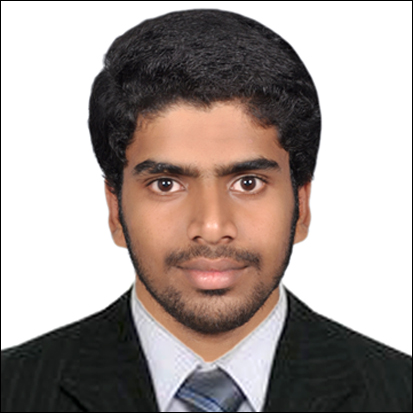
\includegraphics[width=0.6\columnwidth]{my.jpeg}
	\vspace{-8cm}
\end{figure}

\begin{flushright}\small
	Maliackal (H)
	Mookkannoor
	Angamaly- 683577 
	Kerala \\
	
	
	(+91) 9447827165\\
	\tiny
	\url{akhilmaliackal@gmail.com}  \\
\end{flushright}\normalsize
\framebreak



\Huge\bfseries {\color{RoyalBlue} Akhil Joy} \\


\normalsize\normalfont



\color{RoyalBlue}MY Objective is \color{Black}“To pursue a challenging career in the field of Computer Science and to be a part of progressive organization that provides generous opportunities for learning and advancement in my career.\newline





\CVSection{Education}


\begin{tabular}{ |p{2cm}|p{3cm}|p{4cm}|p{2cm}|p{1.5cm}|}
 \hline
 \vfill 
 
\color{red} Degree&\vfill \color{red}  College/School&\vfill \color{red} University/ Board&\vfill \color{red} Passing Year&\vfill \color{red} Pass Percentage/ CGPA\\
 \hline \vfill
 Under graduate (B tech) & \vfill Federal Institute of Science And Technology &\vfill APJ Abdul Kalam Technological University&\vfill 2019&\vfill 7.8\tiny cgpa\\
 \hline \vfill
 XII & \vfill Govt Higher Secondary School Manjapra  &\vfill State Board&\vfill 2015&\vfill 82.58\% \\\hline
  \vfill X &\vfill De Paul EMHSS Angamaly & \vfill State Board &\vfill 2013 &\vfill 94\% \\\hline


 
\end{tabular}
\newline \newline
\sep

\CVSection{  Projects}

\begin{enumerate}
    \item \color{RoyalBlue}Maze solving Bot using reinforcement learning\color{Black}
    \newline \scriptsize Developed a Bot which can solve any kind of  given maze in shortest period of time. It has been developed by using reinforcement learning technique. Initially the Bot traverse  the entire maze and it creates a graph structure internally which simulate the real world by taking this as input. The Bot apply SARSA algorithm to find out the shortest path.
    \item \normalsize \color{RoyalBlue}Hospital Outpatient ticket-booking system\color{Black}
    \newline  \scriptsize Developed a common platform called ”helloDoc” which enables a direct
communication between patient and hospitals. It helps the patient to find
out the best hospital and doctors in his locality and to book the OP tickets and thereby helps in getting a good medical treatment.
\end{enumerate}
\sep




\CVSection{Training and Internship}
\begin{compactitem}[\color{RoyalBlue}$\circ$]
	\item \normalsize \color{RoyalBlue} Aabasfot Technologies (India) Pvt.Ltd.\color{black}\hfill \tiny Kochi, Kerala\normalsize
	\newline 
	\scriptsize Worked on the following technologies: \hfill \tiny June 2017\normalsize
        	\begin{itemize}
          \item \scriptsize Java Basics
          \item \scriptsize Introduction to Android
          \item \scriptsize  Application Development
        \end{itemize}
        
	\item \normalsize \color{RoyalBlue}FISAT Summer school\color{black} \hfill \tiny Angmaly, kerala\normalsize
		\newline 
	\scriptsize Worked on the following technologies: \hfill \tiny May 2016 - July 201\normalsize
        	\begin{itemize}

          \item \scriptsize Machine learning
          \item \scriptsize Game Development
                  \end{itemize}
\end{compactitem}

\sep
         \clearpage
\framebreak
\framebreak




\CVSection{Research Publications}

\begin{enumerate}
 \item \color{RoyalBlue}Artificial Intelligence in Power Systems\color{Black}
 \newline \scriptsize Presented paper based on the application level importance of Artificial Intelligence in power systems which helps in  fault detection and to reduce complexity in Power Systems. Paper  was presented at National level Technical Festival at Viswajyothi College of Engineering and Technology 
 \item \normalsize  \color{RoyalBlue}Intelligent Diagnosis of Diseases\color{Black}
 \newline \scriptsize Presented paper based on techniques that helps to identify most of common diseases without the help of a doctor. It works by taking certain vitals and by applying machine learning algorithms, Paper was  presented at National conference on Emerging Technologies at MES college of Engineering and Technology. 
 \end{enumerate}
\Sep



\CVSection{Technical Skills}
\begin{compactitem}[\color{RoyalBlue}$\circ$]
	\item \normalsize \color{RoyalBlue} Programming Languages\color{black}

        	\begin{itemize}
         \scriptsize \item  C
        \scriptsize  \item C++
       \scriptsize   \item Python 
       \scriptsize   \item  Java 
           \item Assembly language
          \item PHP
            \item AWK
          \item Java Script
     
        \end{itemize}
        
	\item \normalsize \color{RoyalBlue}Platforms\color{black}
	
        \scriptsize	\begin{itemize}
          \item Android Studio
          \item Arduino
          \item laTex
          \item Atmega Studio
          \item PyQt
          
        \end{itemize}
    
    	\item \normalsize \color{RoyalBlue}Database\color{black}
	
        	\begin{itemize}
         \scriptsize \item SQL\newline\newline
        
          
                  \end{itemize}
\end{compactitem}


\end{document}